% !TEX root = pfe-book1.tex
%!TEX TS-program = pdflatex
%!TEX encoding = UTF-8 Unicode


\cleardoublepage
\chapter{ Conservation Laws}
\section{Recoil}
Even those who have not been at war know that when
a gun is fired it jumps back abruptly. When a rifle is
fired, recoil in the shoulder occurs. But it is possible
to become acquainted with recoil without having recourse
to firearms. Pour some water into a test tube, cork it up
and suspend it horizontally on two threads (\figr{fig-3.01}).
Now turn on a burner under the test tube, the water will
begin boiling, and in a couple of minutes the cork will
fly out in one direction, while the test tube will be deflected in the opposite direction.

The force which drove the cork out of the test tube is
steam pressure. And the force deflecting the test tube is
also steam pressure. Both motions arose under the action
of one and the same force. The same thing also happens in
shooting, only there the action is not that of steam but
of gunpowder gas.
\begin{figure}[!ht]
\centering
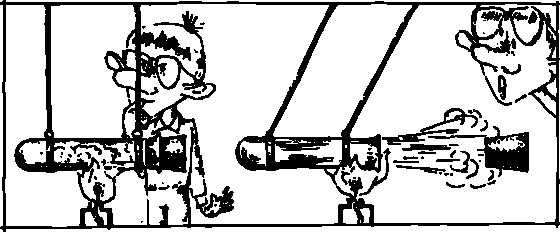
\includegraphics[width=\textwidth]{figures/fig-03-01.pdf}
\caption{The action and reaction.}
\label{fig-3.01}
\end{figure}

Recoil is an inevitable consequence of the principle
of equality between an action and its reaction. If the
steam acts on the cork, the cork also acts on the steam
in the opposite direction, and the steam transmits this
reaction to the test tube.

Perhaps the following objection occurs to you: Can one
and the same force really lead to such dissimilar effects?
The rifle moves backwards only slightly, but the bullet
flies far away. We hope, however, that such an objection
had not occurred to the reader. Identical forces certainly
can lead to different effects: for the acceleration which
a body receives (and this is precisely the effect of the
action of the force) is inversely proportional to its mass.
We must write out the acceleration of one of the bodies
(shell, bullet, cork) in the form $a_{1} = F/m_{1}$; the acceleration of the body experiencing recoil (gun, rifle, test tube) is then $a_{2} = F/m_{2}$ Since the force is one and the same, we arrive at an important conclusion: the accelerations imparted by the interaction of two bodies participating in a ``shot'' will be inversely proportional to their masses:
\begin{equation*}%
\frac{a_{1}}{a_{2}} = \frac{m_{2}}{m_{1}}
\end{equation*}
This means that the acceleration imparted to the gun
when it recoils will be as many times less than the acceleration of the shell as the gun weighs more than the
shell.

The acceleration of the bullet, and also of the rifle
during recoil, lasts as long as the bullet is moving through
the muzzle. Let us denote this time by $t$. When this time
has elapsed, the accelerated motion will become uniform.

For the sake of simplicity, we shall assume the acceleration to be constant. Then the speed with which the bullet flies out of the muzzle of the rifle is $v_{1} = a_{1}t$, and the speed of recoil is $v_{2}= a_{2}t$. Since the time during which the accelerations act is one and the same, then $ v_{1}/v_{2} = a_{1}/a_{2}$, and so
\begin{equation*}%
\frac{v_{1}}{v_{2}} = \frac{m_{2}}{m_{1}}
\end{equation*}
The speeds with which the bodies fly apart after the interaction will be inversely proportional to their masses.

If we recall the vector nature of velocity, we can rewrite the last relation as follows:
\begin{equation*}%
m_{1}\mathbf{v_{1}} = - m_{2}\mathbf{v_{2}}
\end{equation*}
the minus sign indicates that the velocities $\mathbf{v_{1}}$ and $\mathbf{v_{2}}$ are oppositely directed.

Finally, let us rewrite our equation once again bringing the products of mass by velocity to one side:
\begin{equation*}%
m_{1}\mathbf{v_{1}} + m_{2}\mathbf{v_{2}} = 0
\end{equation*}


\section{The Law of Conservation of Momentum}

The product of the mass of a body by its velocity is
called the \emph{momentum} of the body (another name for it is
\emph{linear momentum}). Since velocity is a vector, momentum
Is also a vector quantity. Of course, the direction of the
momentum coincides with that of the velocity of motion
of the body.

With the aid of our new concept, Newton's law, $F = ma$, can be expressed differently. Since $a =(v_{2} - v_{1})/t$,
we have $F =(mv_{2} - mv_{1})/t$, or 
\begin{equation*}%
Ft = mv_{2} - mv_{1}
\end{equation*}
The product of the force by the duration of its action is equal
to the change in the momentum of the body.

Let us return to recoil.

The result of our investigation of the recoil of a gun
can now be formulated more concisely: the sum of the
momenta of the gun and the shell will remain equal to
zero after the firing. It is obvious that this was also the
case before the firing, when the gun and the shell were
in a state of rest.

The velocities occurring in the equation $m_{1}\mathbf{v_{1}} +
m_{2}\mathbf{v_{2}} = 0$ are the velocities immediately after the
firing. During the subsequent motion of the shell and
the gun, the force of gravity and air resistance will begin
acting on them, and the Earth will exert an additional
frictional force on the gun. But if the shot were fired in
a vacuum from a gun hanging in the void, the motion
with the velocities $\mathbf{v_{1}}$ and $\mathbf{v_{2}}$ would continue arbitrarily long. The gun would move in one direction, and the shell in the opposite direction.

Guns mounted on a platform and firing while in motion
are widely applied in current artillery practice. How
should the equation we derived be changed in order that
it be applicable to a shot fired from such a gun? We may
write:
\begin{equation*}%
m_{1}\mathbf{u_{1}} + m_{2}\mathbf{u_{2}} = 0
\end{equation*}
where $\mathbf{u_{1}}$ and $\mathbf{u_{2}}$ are the velocities of the shell and the gun relative to the moving platform. If the velocity of the platform is $\mathbf{V}$, then the velocities of the shell and the
gun relative to an observer who is at rest will be 
\begin{align*}%
\mathbf{v_{1}} & = \mathbf{u_{1}}  + \mathbf{V} \,\, \textrm{and}\\
\mathbf{v_{2}} & = \mathbf{u_{2}}  + \mathbf{V}
\end{align*}
Substituting for $\mathbf{u_{1}}$ and $\mathbf{u_{2}}$ in our previous equation, we
obtain:
\begin{equation*}%
(m_{1} + m_{2}) \, \mathbf{V} = m_{1}\mathbf{v_{1}} + m_{2}\mathbf{v_{2}}
\end{equation*}
In the right-hand side of the equation we have the sum
of the momenta of the shell and the gun after the firing.
And in the left-hand side? Before the firing, the gun and
the shell with a total mass of $m_{1}+ m_{2}$ move together with the velocity $\mathbf{V}$. Therefore, in the left-hand side of
the equation there is also the total momentum of the shell
and the gun, but before the firing.

We have proved a very important law of nature, which
is called the \emph{law of conservation of momentum}. We proved
it for two bodies, but it can easily be proved that the
same result also holds for any number of bodies. What is
the content of this law? The law of conservation of momentum asserts that the sum of the momenta of a number
of interacting bodies does not change as a result of this
interaction.

It is clear that the law of conservation of momentum
will only be valid when no outside forces are exerted on
the group of bodies under consideration. Such a group of
bodies is called closed in physics.

A rifle and a bullet behave like a closed group of two
bodies during a shooting in spite of the fact that they
are subject to the Earth's gravitation. The weight of
the bullet is small in comparison with the force exerted
by gunpowder gases, and recoil occurs in accordance with
one and the same laws, regardless of where the shot will
be fired -- on the Earth or in a rocket flying through interplanetary space.

The law of conservation of momentum allows us to
easily solve various problems dealing with colliding
bodies. Let us try to strike one clay ball with another -- they will stick together and continue the motion together;
if we shoot from a rifle at a wooden ball, it will roll together with the bullet stuck in it; a standing cart will roll
if a person takes a running jump into it. All the examples
we have given are very similar from the point of view of
physics. The rule relating the velocities of the bodies
involved in such kinds of collisions can be immediately
obtained from the law of conservation of momentum.
\begin{figure}[!ht]
\centering
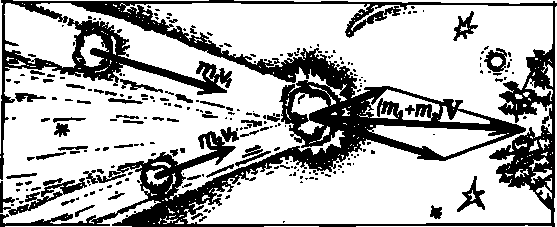
\includegraphics[width=\textwidth]{figures/fig-03-02.pdf}
\caption{The law of conservation of momentum.}
\label{fig-3.02}
\end{figure}

The momenta of the bodies prior to their collision were
$m_{1}\mathbf{v_{1}}$ and $m_{2}\mathbf{v_{2}}$ they united after the collision, and their total mass is equal to $m_{1} + m_{2}$. Denoting the velocity of the united body by $\mathbf{V}$, we obtain:
\begin{align*}%
m_{1}\mathbf{v_{1}} + m_{2}\mathbf{v_{2}} & = (m_{1} + m_{2})\, \mathbf{V} \,\, \textrm{or}\\
\mathbf{V} & = \frac{m_{1}\mathbf{v_{1}} + m_{2}\mathbf{v_{2}}}{m_{1} + m_{2}}
\end{align*}
Let us recall the vector nature of the law of conservation
of momentum. The momenta $m\mathbf{v}$ in the numerator of the
formula must be added like vectors.

The ``uniting hit'' when bodies moving at an angle to
each other meet is shown in \figr{fig-3.02}. In order to find
the speed, we must divide the length of a diagonal of the
parallelogram formed by the momentum vectors of the
colliding bodies by the sum of their masses.

\section{Jet Propulsion}

A person moves by pushing off from the Earth; a boat
sails because the rowers push against the water with their
oars; a ship also pushes against the water, only not with
oars but with propellers; a train moving on rails and an
automobile also push off from the Earth -- remember how
hard it is for an automobile to get started on an icy road.
Thus, pushing off from a support seems to be a necessary
condition for motion; even an airplane moves by pushing
the air with its propeller.


But is it really? Might there not be some intricate
means of moving without pushing off from anything. If
you ice-skate, you can easily convince yourself on the
basis of your experience that such motion is quite possible. Pick up a heavy stick and get on the ice. Throw the stick forward -- what will happen? You will glide backwards, although the thought of pushing against the ice with your foot didn't even cross your mind.

Recoil, which we have just studied, yields us the clue
to carrying out motion without support, without pushing
off. Recoil presents a possibility of accelerating motion
even in a vacuum, where there really is absolutely nothing
to push off from.
\begin{figure}[!ht]
\centering
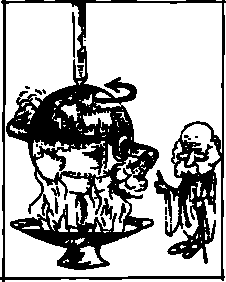
\includegraphics[width=0.6\textwidth]{figures/fig-03-03.pdf}
\caption{An ancient steam turbine.}
\label{fig-3.03}
\end{figure}

The recoil caused by a steam jet being driven out of
a vessel (the reaction of the jet) was used back in Ancient
Times for creating curious toys. An ancient steam turbine
invented in the second century B.C. is pictured in \figr{fig-3.03}. A spherical cauldron was supported by a vertical axis. Escaping from the cauldron through elbow-shaped pipes, the steam pushed these pipes in the opposite direction, and the sphere rotated.

These days the use of jet propulsion has already gone
far beyond the realm of the creation of toys and the collection of interesting observations. The twentieth century
is sometimes called the century of atomic energy, but
with no less reason one could call it the century of jet
propulsion, since the far-reaching consequences of the
use of powerful jet engines can scarcely be exaggerated. This is not only a revolution in aircraft construction but
the beginning of mankind's contact with the Universe.

The principle of jet propulsion permits the creation
of airplanes moving with a speed of several thousand
kilometres per hour, flying missiles rising hundreds of
kilometres above the Earth, artificial Earth satellites and
cosmic rockets carrying out interplanetary flights.

A jet engine is a machine from which gases formed by
the combustion of fuel are ejected with great force. The
rocket moves in the direction opposite to that of the gas
stream.

How strong is the thrust carrying the rocket off into
space? We know that the force is equal to the change in
momentum during a unit of time. According to our conservation law, the momentum of the rocket changes by the total momentum $mv$ of the ejected gas.

This law of nature allows us to compute, for example,
the relation between the force of the jet propulsion and
the expenditure of fuel necessary for this. In doing so,
one must assume a value for the speed of discharge of the
combustion products. 

Let us take, say, the following values: the gases are ejected with a speed of \SI{2000}{\meter\per\second} at the rate of 10 tons per second. Then the force in the jet propulsion will be about \num{2d12}~dyn, i.e. approximately \num{2000}~tonf.

Let us determine the change in speed of a rocket moving
in interplanetary space.

The momentum of the mass $\Delta M$ of gas ejected with
speed $u$ is equal to $u \Delta M$. The momentum of a rocket of
mass $M$ will increase by the amount $M \Delta V$. According
to our conservation law, these two quantities must be
equal to each other:
\begin{equation*}%
u \Delta M = M \Delta V, \,\, \textrm{i.e.} \,\, \Delta V = u \frac{\Delta M}{M}
\end{equation*}
However, if we wish to compute the speed of a rocket
when the ejected mass is comparable to the mass of the
rocket, the formula we have derived turns out to be
useless. In fact, it assumes that the mass of the rocket
is constant. However, the following important result
remains valid: identical relative changes in mass lead
to one and the same change in speed.

A reader acquainted with the basics of integral calculus
will at once obtain the true formula. It has the form
\begin{equation*}%
V = u \ln \frac{M_{in}}{M} = 2.3 \, u \ln \frac{M_{in}}{M}
\label{rocket-eq}
\end{equation*}
If you use a slide rule, you will find that when the mass
of the rocket is cut in half, its speed will reach $0.7u$.

In order to raise the speed of the rocket to $3u$, it is
necessary to burn up a mass $m = (19/20) M$. This means
that only one-twentieth of the mass of the rocket can
be preserved if we wish to raise its speed to $3u$, i.e. to
\SIrange{6}{8}{\kilo\meter\per\second}.

In order to attain a speed of $7u$, the mass of the rocket
must decrease by 1000 times during the speed-up.

These calculations warn us against striving to increase
the mass of the fuel which can be put in the rocket. The
more fuel we take, the more we must burn. For a given
speed of gas ejection, it is very difficult to achieve an
increase in the speed of the rocket.

The increase in the speed of gas ejection is the basic
means of attaining high rocket speeds. In this respect, a significant role must be played by the application to rockets of engines running on a new atomic fuel.

For a constant speed of gas ejection, a gain in speed
with the same mass of fuel is obtained by using multistage rockets. In a single-stage rocket, the mass of the
fuel decreases, but the empty tanks keep moving with
the rocket. An additional energy is required to accelerate
the mass of the unnecessary fuel tanks. It would be
expedient to throwaway the fuel tanks whose fuel has
been consumed. In modern multi-stage rockets, not only
are the fuel tanks and piping thrown away but also the
engines of the used stages.

Of course, it would be best to continuously throwaway
the unnecessary mass of the rocket. Such a construction
does not yet exist. The take-off weight of a three-stage
rocket can be made six times less than that of a single-
stage rocket with the same ``ceiling'' A ``continuous''
rocket would be more profitable in this sense than a three-stage rocket by an additional 15\%.

\section{Motion Under the Action of Gravity}

We shall roll a small cart down two very smooth
inclined planes. Let us take two boards, one much shorter
than the other, and place them on one and the same support. Then one inclined plane will be steep, and the
other will be gently sloping. The tops of both boards -- the starting places of the cart -- will be at the same height.
In which case do you suppose will the cart acquire the
greater speed by rolling down its inclined plane? Many
people will decide that it will be the one which rolls
down the steeper board.
\begin{figure}[!ht]
\centering
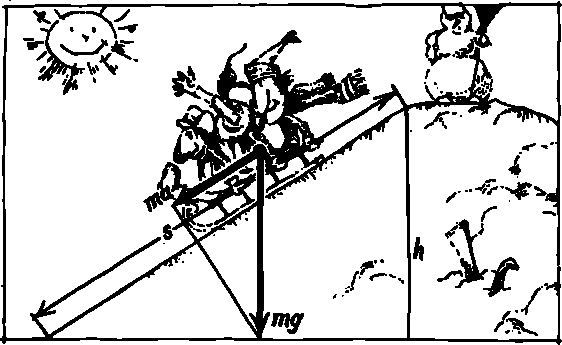
\includegraphics[width=\textwidth]{figures/fig-03-04.pdf}
\caption{Analysing motion of a cart rolling down.}
\label{fig-3.04}
\end{figure}

An experiment will show that they are wrong -- in both
cases the cart will acquire the same speed. While a body
is moving along an inclined plane, it is subject to the
action of a constant force? namely (\figr{fig-3.04}), the component of gravity directed along the line of its motion. The speed $v$ which a body acquires moving with acceleration a along a path of length $s$ is equal, as we know, to $\sqrt{2as}$.

What makes it evident that this magnitude does not
depend on the angle of inclination of the plane? We see
two triangles in \figr{fig-3.04}. One of them depicts the
inclined plane. The small leg of this triangle denoted by
$h$ is the height from which the motion begins; the hypotenuse $s$ is the path through which the body passes in its
accelerated motion. The small force triangle with leg
$ma$ and hypotenuse $mg$ is similar to the large one, since
they are right triangles, and their angles as angles with
mutually perpendicular sides are equal. Hence, the ratio
of the legs should be equal to that of the hypotenuses, i.e,
\begin{equation*}%
\frac{h}{ma} = \frac{s}{mg} \,\, \textrm{or} \,\,  as = gh
\end{equation*}
We have proved that the product $as$, and hence the
final speed of a body rolling down an inclined plane, is
independent of the angle of inclination but depends only
on the height from which the downward motion began.
The speed $v = \sqrt{2gh}$ for all inclined planes subject to the
sole condition that the motion began from one and the
same height $h$. This speed turned out to be equal to the
speed of free fall from height $h$.

Let us measure the speed of a body at two places on
the inclined plane -- at heights $h_{1}$ and $h_{2}$. Denote the
speed of the body when it passes through the first point
by $v_{1}$ and its speed when it passes through the second
point by $v_{2}$.

If the initial height from which the motion began is $h$,
the square of the speed of the body at the first point
will be $v_{1}^{2} = 2g (h - h_{1})$ and at the second point $v_{2}^{2}= 2g (h - h_{2})$. Subtracting the former from the latter,
we shall find out how the speeds of the body at the initial
and end points of an arbitrary piece of an inclined plane
are related to the heights of these points:
\begin{equation*}%
v_{2}^{2} - v_{1}^{2} = 2g (h_{1} - h_{2})
\end{equation*}
The difference between the squares of the speeds depends
only on the difference in height. Note that the equation
we have obtained is equally suitable for upward motion
and downward motion. If the first height is less than the
second (ascent), the second speed is less than the first.

This formula can be rewritten in the following way:
\begin{equation*}%
v_{2}^{2} - v_{1}^{2} = 2g (h_{1} - h_{2})
\end{equation*}
We wish to emphasize by means of this formulation
that the sum of half the square of the speed and g times
the height is identical for all the points on the inclined
plane. One may say that the quantity $(v^{2}/2) + gh$ is conserved during the motion.

What is most remarkable in the law we have found is
that it is valid for frictionless motion on any hill and,
in general, along any path consisting of alternating
ascents and descents of various slopes. This follows from
the fact that any path can be broken up into rectilinear
portions. The smaller we take the segments, the closer
will the broken line approximate the curve. Each straight
line segment into which the curvilinear path has been
broken up may be regarded as part of an inclined plane,
and the rule we have found may be applied to it.

Therefore, the sum $(v^{2}/2) + gh$ is identical for all the points of the trajectory. Consequently, a change in the square of the speed does not depend on the form or length of the path along which a body moved but is determined solely by the difference in height of the initial and end points of the motion.

It may seem to the reader that our conclusion does not
coincide with his daily experience: on a long, gently
sloping path a body does not gather any speed at all,
and eventually comes to a halt. This is the way things are,
but we haven't taken the force of friction into account
in our reasoning. The above formula is valid for motion
within the Earth's gravitational field under the action of
only the single force of gravity. If the frictional force
is small, the derived law will be satisfied rather well.
A sled with metal runners slides down smooth icy mountains with very little friction. It is possible to build
long icy paths that begin with a steep descent on which
a great speed is gathered and then twist up and down
fantastically. The end of a trip on such a hill (when the
sled stops by itself) would occur at a height equal to
that of the start, provided that friction were entirely
absent. But since it is impossible to avoid friction, the
point at which the motion of the sled started will be
higher than the place where it stops.

The law which asserts that the final speed pf a motion subject to the force of gravity is independent of the form of the path can be applied to the solution of various interesting problems.

``Looping-the-loop'' in a vertical circle has been frequently presented at circuses as an exciting stunt. A cyclist or a cart with an acrobat in it is placed on a high
platform. He then accelerates while descending. Now
he is ascending. Look, he is in an upside-down position.
then again a descent, and the loop has been looped. Let
us consider a problem which a circus engineer must solve.
At what height should the platform from which the descent begins be made, so that the acrobat might loop-the-loop within falling? We know a necessary condition:
the centrifugal force pressing the acrobat against the cart
must balance the oppositely directed gravitational force.

Hence $mg \leqslant mv^{2}/r$, where $r$ is the radius of the loop,
and $v$ is the speed of the motion at the top of the loop.
In order that this speed be attained, it is necessary to
begin the motion from a place which is a certain quantity
$h$ higher than the top of the loop. Since the initial speed
of the acrobat is equal to zero, we have $v^{2} = 2gh$ at the
top of the loop. But, on the other hand, $v^{2} \geqslant gr$. Hence,
between the height $h$ and the radius of the loop there is
the relation $h \geqslant r/2$. The platform must be raised by
at least half the radius of the loop above the top of the
loop. Taking into account the inevitable frictional force,
we shall, of course, have to choose our height with a margin of safety.

And here is another problem. Let us take a large, very
smooth dome so that friction is minimum. Let us place
a small object at the top and give it the opportunity
of sliding down the dome by means of hardly noticeable
push. Sooner or later the sliding body will get detached
from the dome and start falling. We can easily answer the
question as to just when the body breaks away from the
surface of the dome: at the moment of the break the
centrifugal force must equal the radial component of
the weight (at this instant the body will cease pressing
the dome, and this is precisely the moment of the break).
Two similar triangles can be seen in \figr{fig-3.05}; the
moment of the break is depicted. Let us form the ratio
of a leg to the hypotenuse for the force triangle and set
it equal to the corresponding ratio for the other triangle:
\begin{equation*}%
\frac{mv^{2}/r}{mg} = \frac{r-h}{r}
\end{equation*}
\begin{figure}[!ht]
\centering
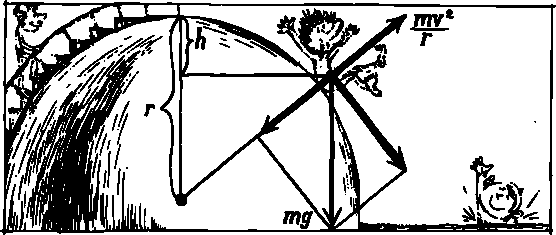
\includegraphics[width=\textwidth]{figures/fig-03-05.pdf}
\caption{Analysing motion of an object sliding down a dome.}
\label{fig-3.05}
\end{figure}

Here $r$ is the radius of the spherical dome, and $h$ is the
difference in height between the start and finish of the
sliding. Let us now make use of the independence of the
final speed of the form of the path. Since the initial
speed of a body is assumed equal to zero, we have $v^{2} =
 2gh$. Substituting this value in the above proportion
and performing arithmetical transformations, we find
$h = r/3$. Hence, the body will break away from the dome
at a height which is one-third of a radius lower than the
top of the dome.

\section{The Law of Conservation of Mechanical Energy}

We have convinced ourselves in the examples just considered how helpful it is to know a quantity not changing
its numerical value (conserving it) throughout a motion.

So far we know such a quantity for one body only. But
if several associated bodies are moving within a gravitational field? It is evident that we may not assume that
the expression $(v^{2}/2) + gh$ remains constant for each
of them, since each of the bodies is subject to the action
of not only the force of gravity but also of the neighbouring bodies. Perhaps the sum of such expressions taken over the group of bodies under consideration is conserved?

We shall now show that this assumption is false. There
exists a quantity conserved throughout the motion of
many bodies; however, it is not equal to the sum
\begin{equation*}%
\left( v^{2} + gh \right)_{\textrm{body\,1}}+
\left( v^{2} + gh \right)_{\textrm{body\,2}} + \ldots
\end{equation*}
but rather to the sum of such expressions multiplied by
the masses of the corresponding bodies; in other words,
the sum
\begin{equation*}%
m_{1}\left( v^{2} + gh \right)_{1}+
m_{2}\left( v^{2} + gh \right)_{2}+ \ldots
\end{equation*}
is conserved.

For the proof of this important law of mechanics, we
turn to the following example.

Two loads are connected by a cord passing over a pulley, the large one of mass $M$, and the small one of mass $m$. The large load pulls the small one, and this group of two bodies will move with increasing speed.

The driving force is the difference in weight of these bodies, $Mg - mg$. Since the masses of both bodies participate in the accelerated motion, Newton's law for this case will be written out as follows:
\begin{equation*}%
(M-m)g = (M+m)g
\end{equation*}
Let us consider two instants during the motion and
show that the sum of the expressions $(v^{2}/2) + gh$ multiplied by the corresponding masses really remains unchanged. Thus, it is required to prove the equality
\begin{equation*}%
m\left( v_{2}^{2} + gh_{2} \right)+
M\left( V_{2}^{2} + gH_{2} \right)
= m\left( v_{1}^{2} + gh_{1} \right)+
M\left( V_{1}^{2} + gH_{1} \right)
\end{equation*}
Capital letters denote physical quantities characterizing
the large load. The subscripts 1 and 2 refer here to the
two instants which we are considering.

Since the loads are connected by a cord, $v_{1} = V_{1}$ and
$v_{2} = V_{2}$. Using these simplifications and transferring
all summands containing heights to the right-hand side,
and summands with speeds to the left-hand side, we
obtain:
\begin{align*}%
\frac{m+M}{2} (v_{2}^{2}-v_{1}^{2}) & = mgh_{1}+MgH_{1}-mgh_{2}-MgH_{2}\\
& = mg(h_{1}-h_{2}) + Mg(H_{1}-H_{2})
\end{align*}
The differences in height of the loads are, of course,
equal (but opposite in sign since one load rises and the other falls). Therefore,
\begin{equation*}%
\frac{m+M}{2} (v_{2}^{2}-v_{1}^{2}) = g(M - m)s
\end{equation*}
where $s$ is the distance covered.

We learned on p.~\pageref{dist-time-acc} that the difference between the squares of the speeds at the initial and end points of a
segment of length $s$ of a path traversed with acceleration $a$ is equal to:
\begin{equation*}%
v_{1}^{2}-v_{2}^{2} = 2as
\end{equation*}
Substituting this expression in the preceding formula, we find:
\begin{equation*}%
(m + M) a = (M - m) g
\end{equation*}
But this is Newton's law, which we have written out
above for our example. With this we have proved what
was required: for two bodies the sum of the expressions
$(v^{2} /2) +gh$ multiplied by the corresponding masses\footnote{Of course, the expression $(v^{2} / 2) +gh$ could equally well be multiplied by $2m$, or $m/2$, and, more generally, by an arbitrary factor. We agreed to act in the simplest manner, i.e. to multiply it simply by $m$.} remains constant during the motion, or, as one says, is conserved, i.e.
\begin{equation*}%
\left(\frac{mv^{2}}{2} + mgh\right) + \left(\frac{MV^{2}}{2} + MgH\right) = \textrm{const.}
\end{equation*}

For the case of a single body, this formula reduces to
the one proved earlier:
\begin{equation*}%
\frac{v^{2}}{2} + gh = \textrm{const.}
\end{equation*}
Half the product of the mass by the square of the speed
is called the \emph{kinetic energy} $K$:
\begin{equation*}%
K = \frac{mv^{2}}{2}
\end{equation*}
The product of the weight of a body by its height is
called the \emph{potential energy} $U$ of the gravitational attraction of the body to the Earth:
\begin{equation*}%
U = mgh
\end{equation*}
We have proved that during the motion of a two-body
system (and it is possible to prove the same thing for a
system consisting of many bodies) the sum of the kinetic
and potential energies of the bodies remains constant.
In other words, an increase in the kinetic energy of a
group of bodies can only occur at the expense of a decrease
in the potential energy of this system (and, of course,
conversely).

The law just proved is called the \emph{law of conservation
of mechanical energy}.

The law of conservation of mechanical energy is a very
important law of nature. We have not yet shown its significance in full measure. Later, when we have become acquainted with the motion of molecules, its universality and its applicability to all natural phenomena will be evident.

\section{Work}
If we push or pull a body meeting no hindrance to
what we are doing, the result will be an acceleration of
the body. The increase in kinetic energy taking place in
this connection is called the \emph{work} $A$ performed by the
force:
\begin{equation*}%
A= \frac{mv_{2}^{2}}{2} -  \frac{mv_{1}^{2}}{2}
\end{equation*}
According to Newton's law, the acceleration of a body
and hence also the increase in its kinetic energy, is determined by the vector sum of all the forces applied to it. Therefore, in the case of many forces, the formula $A = (mv_{2}^{2}/2) - (mv_{1}^{2}/2)$ expresses the work performed by the resultant force. Let us express the work $A$ in terms of the magnitude of the force.

For the sake of simplicity, we shall restrict ourselves
to the case when motion is possible only in one direction --
we shall push (or pull) a cart of mass $m$, standing on rails
(\figr{fig-3.06}).
\begin{figure}[!ht]
\centering
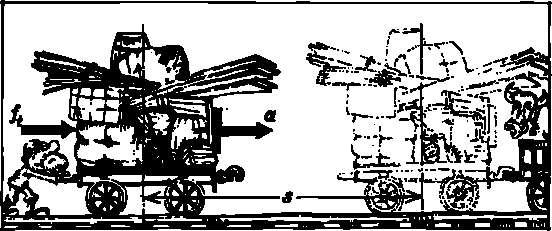
\includegraphics[width=\textwidth]{figures/fig-03-06.pdf}
\caption{Work done to push a cary on rails.}
\label{fig-3.06}
\end{figure}

According to our general formula for uniformly accelerated motion, $v_{2}^{2} - v_{1}^{2} = 2as$. Therefore, the work performed by all the forces over a distance $s$ is
\begin{equation*}%
A= \frac{mv_{2}^{2}}{2} -  \frac{mv_{1}^{2}}{2} = mas
\end{equation*}
The product $ma$ is equal to the component of the total
force in the direction of the motion. Consequently, $A =f_{t}s$.

The work done by a force is measured by the product of
the distance by the component of the force along the
direction of the displacement.

This formula for the work is valid for forces of any
origin and for motions along any trajectory.

Note that the work may be equal to zero even when
forces act on a moving body.

For example, the work done by a Coriolis force is equal
to zero, because such a force is perpendicular to the direction of the motion. It has no tangential component, so the work is equal to zero.

Any twist in the trajectory which is not accompanied
by a change in speed requires no work, for the kinetic energy does not change under such conditions.

Can work be negative? Of course, if the force is directed
at an obtuse angle to the motion, then it does not help
but hinders the motion. The tangential component of the
force in the direction of the motion will be negative. In
this case we do say that the force performs negative work.
The force of friction always slows down a motion, i.e.
does negative work.

On the basis of the increase in kinetic energy, one can
only judge the work done by the resultant force.

As for the work done by the individual forces, we should
compute them as the products $f_{t}s$. An automobile is moving uniformly along a highway. There is no increase in
kinetic energy, so the work done by the resultant force
is equal to zero. But the work done by the motor is, of
course, not equal to zero -- it is equal to the product of
the thrust of the motor by the distance covered, and is
fully compensated by the negative work done by the force
of friction and resistance.

Using the concept of ``work'', we can describe more
briefly and clearly the interesting peculiarities of the
gravitational force with which we have just become acquainted. If a body goes from one place to another under
the action of gravity, its kinetic energy will change. This
change in kinetic energy is equal to the work $A$. But we
know from the law of conservation of energy that an
increase in kinetic energy takes place at the expense of
a decrease in potential one.

Therefore, the work done by gravity is equal to the
decrease in potential energy:
\begin{equation*}%
A = U_{1} - U_{2}
\end{equation*}
It is obvious that a loss (or gain) of potential energy,
and hence an increase (or decrease) in kinetic energy,
will be the same, regardless of the path along which a body
moved. This implies that the work performed by gravity
does not depend on the form of the path. If a body went
from the first point to the second with an increase in
kinetic energy, it will go from the second point to the
first with a decrease in kinetic energy by exactly the same
amount. Moreover, it makes no difference whether or
not the form of the path ``there'' coincides with the form
of the path ``back''. Hence, the work ``there'' and ``back''
will also be identical. And if the body takes a long trip
with the initial and end points of its path coinciding, the
work will be equal to zero.

Imagine a canal whose form is as fantastic as possible,
through which a body slides without friction. Let us send
it off on a trip from the highest point. The body rushes
downwards gathering speed. At the expense of the kinetic energy so obtained, the body will surmount ascents and
return finally to the station where it departed. With
what speed? With the same, of course, with which it
left the station. Its potential energy will return to its
previous value. But if so, then its kinetic energy could
neither have decreased nor increased. Hence, the work
is equal to zero.

Not for all forces is the work done along a circular
(physicists say: a closed) path equal to zero. There is no
need to prove that the longer the path, the greater will
be the work performed by friction, for example.

\section{In What Units Work and Energy Are Measured}

Since work is equal to the change in energy, then work
and energy -- potential as well as kinetic, of course -- are
measured in one and the same units. Work is equal to
the product of a force by a distance. The work done by a
force of one dyne over a distance of one centimetre is
called the erg:
\begin{equation*}%
1\,\textrm{erg} = 1\,\textrm{dyn} \cdot \SI{1}{\centi\meter}
\end{equation*}
This is a very small work. Such a work is performed against
gravity by a mosquito in order to fly from the thumb to
the forefinger of someone's hand. A larger unit of work and
energy used in physics is the joule (\si{\joule}). It is 10 million times as great as an erg:
\begin{equation*}%
\SI{1}{\joule} = \num{d7} \, \textrm{dyn}
\end{equation*}
A unit of work which is quite often used is 1 kilogram-force-metre (\SI{1}{\kgf\meter}). This is the work which a force of
\SI{1}{kgf} performs in a displacement of \SI{1}{\meter}. About this much work is done by a kilogram weight falling off a table to the
floor.

As we know, a force of $\SI{1}{\kgf} = \num{981000} \, \textrm{dyn}$, $\SI{1}{\meter} = \SI{100}{\centi\meter}$. Hence, \SI{1}{\kgf\meter} = \num{9.81d7}\, \textrm{erg} = \SI{9.81}{\joule}. Conversely, $\SI{1}{\joule} = \SI{0.102}{\kgf\meter}$.

The SI system of units requires that we drop the kilogram-force-metre as the unit of work and energy and use the joule instead, \SI{1}{\joule} is the work done by a force of \SI{1}{\newton}
over a distance of \SI{1}{\meter}. Knowing how easily force is defined in this case, one has no difficulty in understanding the reason for the advantages of the SI system of units.

\section{Power and Efficiency of Machines}

To estimate the potential of a machine to perform work
and the consumption of energy, the concept of power was
introduced. \emph{Power} is work per unit time, or the time rate
of doing work.

There are many different units of power. In the cgs
system, the unit is the erg per second (erg/s), One erg
per second, however, is very little power and, hence, not
useful in practical life. A unit in much wider use is the
joule per second, or \emph{watt} (\si{\watt}): $\SI{1}{\watt} = \SI{1} {\joule\per\second} = \num{d7} \textrm{erg/s}$. When this unit is not enough, it is multiplied by a thousand. The new unit is called a \emph{kilowatt}: (\si{\kilo\watt}).

From the early days of technology we have inherited
the unit of power called \emph{horsepower} (hp). This name had
a special meaning at that time. A person buying a 10-horsepower machine would conclude that it took the place of 10 horses, even if he knew nothing of units of power.

Naturally, there are no two horses alike. The first person
to introduce this unit of power apparently thought that
the average horse can do \SI{75}{\kgf\meter} of work per second.
Thus, one horsepower was arbitrarily defined as \SI{75}{\kgf\meter\per\second}. A heavy draught-horse can work at a rate greater than 1~hp; especially when starting. But the power of an average horse is about 0.5~hp. The relation of horsepower to
kilowatt is $1~\textrm{hp} = \SI{0.735}{\kilo\watt}$.

In everyday life and in technology we deal with a
great variety of machines. The motor of the turntable of
a record player has a power output of about \SI{10}{\watt}, the
engine of the Soviet car Volga 100~hp or \SI{73}{\kilo\watt}, and the
engines of the Soviet passenger airliner ``IL-18'' \num{16 000}~hp.
A small electric power station used to supply a cooperative farm with electricity has a power output of about \SI{100}{\kilo\watt}, whereas the Krasnoyarsk hydroelectric plant on the Yenisei river in Siberia has a record power output of 5 million kilowatts.

The units of power we have elaborated on give us a clue
to a unit of work or energy used exclusively for electricity,
namely the kilowatt-hour (\si{\kilo\watt\hour}). A kilowatt-hour is
the work produced by a source with the power output of one kilowatt in the course of one hour. From this new unit it is easy to transfer to the old ones: 
\begin{align*}%
\SI{1}{\kilo\watt\hour} & = \SI{3.6d6}{\joule}\\
& = \SI{861}{\kilo\calorie} = \SI{367 000}{\kgf\meter}
\end{align*}

But with so many units of energy was there any need
to introduce one more? Yes, there was. The idea of energy
is used in a great variety of fields of physics, so for the
sake of convenience physicists introduced a new unit for
each field. The same happened with other units of measurement. Finally, there appeared a need for a unified
system of units (the SI system) for all fields of physics.
Some time will have to pass, however, before the ``old''
units will make way for the favoured one, the joule. The
kilowatt-hour is thus not thelast ``outsider'' that the reader
will meet in his study of physics.

What are machines needed for? Obviously, to use sources
of energy to do work: to lift loads, move other machines,
or transport cargo or passengers. For any machine the
amount of energy supplied to it and the output work done
by it can be calculated. In all cases the work output is
less than the work input: part of the energy is lost in
the machine. The ratio of the work output for any machine to the work input is called \emph{efficiency} and is usually
expressed in percent. For example, a machine whose
efficiency is 90 percent loses only 10 percent of the input energy. On the other hand, an efficiency of 10 percent
means that the machine uses only 10 percent of the input
energy.

The efficiency of a machine that transforms mechanical
energy into work can be made very high if the unavoidable
friction is reduced. We can bring the efficiency closer to
100 percent by improving lubrication, using better bearings, reducing the resistance of the medium in which the
movement takes place, etc.

When mechanical energy is transformed into work,
there is often an intermediate stage (as in hydroelectric
plants), namely transmission of electric energy. Naturally,
this stage introduces new losses. But these are small, so
that even when this stage is present, the total loss in
transforming mechanical energy into work can be brought
down to a small percentage.

\section{Energy Loss}

The reader has probably noticed that while illustrating
the law of conservation of mechanical energy we persistently repeat: ``in the absence of friction, if there were
no friction \ldots'' But friction inevitably accompanies any
motion. What is the significance of a law which doesn't
take into account such an important practical circumstance? We shall put off answering this question and consider now some consequences of friction.

Frictional forces are directed against motion, and so
perform negative work. This causes an unavoidable loss
of mechanical energy.

Will this inevitable loss of mechanical energy lead to
a cessation of the motion? It is not difficult to convince
oneself that not every motion can be stopped by friction.

Imagine a closed system consisting of several interacting bodies. The law of conservation of momentum is
valid, as we know, in relation to such a closed system. A
closed system cannot change its momentum, so it moves
rectilinearly and uniformly. Friction within such a system can change relative motions of parts of the system,
but cannot affect the speed and direction of the motion
of the entire system as a whole.

There exists still another law of nature, called the \emph{law
of conservation of angular momentum} (we shall make its
acquaintance later), which does not permit friction to
destroy the uniform rotation of an entire closed system.
Therefore, the presence of friction leads to the cessation of all motions within a closed system of bodies, not
obstructing only the uniform rectilinear and the uniform
rotational motion of this system as a whole.

If the Earth does slightly change the speed of its rotation, the cause of this is not the friction exerted by terrestrial bodies against one another, but the fact that the Earth is not an isolated system.

As for the motions of bodies on the Earth, they are
all subject to friction and lose their mechanical energy.
Therefore, such motion will always cease if not supported
from without.

This is a law of nature. But if one suceeded in tricking
nature? Then \ldots{} then one might be able to bring about
perpetuum mobile, which is Latin for ``perpetual motion''.

\section{Perpetuum Mobile}

Bertold, a hero of Pushkin's \emph{Scenes from the Days of
Knighthood}, dreamed of bringing about perpetuum mobile.

``What is perpetuum mobile?'' asks his interlocutor. ``It
is perpetual motion,'' answers Bertold. ``If I find perpetual motion, I see no bounds to human creativity. To make gold is a tempting problem, a discovery can be curious and profitable, but to find a solution to the problem of perpetuum mobile \ldots{}''

Perpetuum mobile, or a perpetual motion machine, is
a machine working not only contrary to the law of loss of
mechanical energy, but also in violation of the law of
conservation of mechanical energy, which, as we now
know, holds only under ideal unattainable conditions -- in
the absence of friction. A perpetual motion machine must,
as soon as it is constructed, begin working ``by itself'',
for example, turning a wheel or lifting up a load. This
work should take place perpetually and continually, and
the machine should require neither fuel nor human hands
nor the energy of falling water -- in short, nothing got
from without.

The earliest reliable document known so far dealing
with the ``realization'' of a perpetual motion machine
goes back to the 13th century. It is a curious fact that
after six centuries, in 1910, exactly the same ``project''
was presented for ``consideration'' in one of Moscow's
scientific institutions.

\begin{figure}[!ht]
\centering
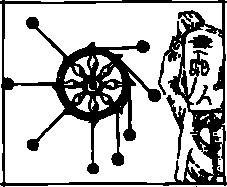
\includegraphics[width=0.6\textwidth]{figures/fig-03-07.pdf}
\caption{An example of perpetual motion machine.}
\label{fig-3.07}
\end{figure}

The project for this perpetual motion machine is depicted in \figr{fig-3.07}. As the wheel rotates, the loads are
thrown back and, according to the inventor, support the
motion, since these loads, acting at a greater distance from the axis, press down much harder than the others. Having constructed this by no means complicated ``machine'', the inventor convinces himself that after turning once or twice by inertia, the wheel comes to a halt. But this does not make him lose heart. An error has been committed: the levers should have been made longer, the protuberances must be changed in form. And the fruitless labour to which many self-made inventors have devoted their lives continues, but of course with the same success.
\begin{figure}[!ht]
\centering
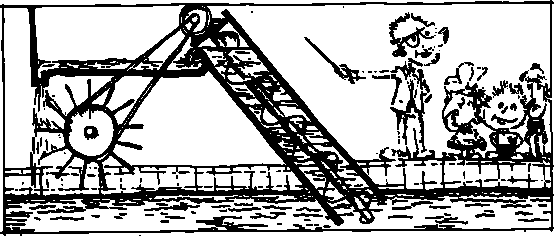
\includegraphics[width=\textwidth]{figures/fig-03-08.pdf}
\caption{An example of perpetual motion machine.}
\label{fig-3.08}
\end{figure}
On the whole, there have not been many variants of
proposed perpetual motion machines: various self-moving
wheels not differing in principle from the one described;
hydraulic machines, for example, the machine shown in
\figr{fig-3.08}, which was invented in 1634; machines using
siphons or capillary tubes (\figr{fig-3.09}), the loss of weight
in water (\figr{fig-3.10}) or the attraction of iron bodies to
magnets. It is by no means always possible to guess at
the expense of what, according to the inventor, the perpetual motion should have occurred.
\begin{figure}[!ht]
\centering
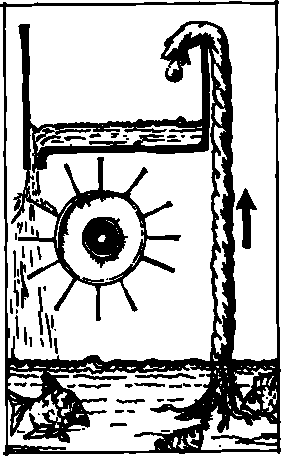
\includegraphics[width=0.5\textwidth]{figures/fig-03-09.pdf}
\caption{An example of perpetual motion machine.}
\label{fig-3.09}
\end{figure}
Even before the law of conservation of energy was established, we find the assertion of the impossibility of perpetuum mobile in an official declaration of the French Academy, made in 1775, when it decided not to accept any more projects for perpetual motion machines to be examined and tested.
\begin{figure}[!ht]
\centering
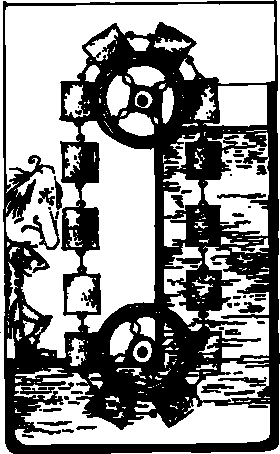
\includegraphics[height=0.6\textheight]{figures/fig-03-10.pdf}
\caption{An example of perpetual motion machine.}
\label{fig-3.10}
\end{figure}


Many $17^{\textrm{th}}$ and $18^{\textrm{th}}$ century physicists had already
assumed the axiom of the impossibility of perpetuum mobile as a basis of their proofs, in spite of the fact that the
concept of energy and the law of conservation of energy
entered science much later.

At the present time it is clear that inventors who try
to create a perpetual motion machine not only come into contradiction with experiment, but also commit an error
in elementary logic, for the impossibility of perpetuum
mobile is a direct consequence of the laws of mechanics, which is what they proceed from in justifying their ``inventions''.

In spite of their complete fruitlessness, searches for
perpetual motion machines probably played, nevertheless, some sort of useful role, since they led in the final analysis to the discovery of the law of conservation of energy.


\section{Collisions}
Momentum is conserved in every collision between two
bodies. As for energy, it will necessarily decrease, as we
have just explained, because of various kinds of friction.

However, if the colliding bodies are made of elastic
material, say of ivory or steel, the energy loss will be
insignificant. Such collisions, for which the sums of the
kinetic energies before and after the collision are identical, are called \emph{ideally elastic}.

A small loss of kinetic energy takes place even in collisions of the most elastic materials; it reaches, for example,
3-4\% with ivory billiard balls.

The conservation of kinetic energy in elastic collisions
permits us to solve a number of problems.

Consider, for example, a head-on collision between
balls of different mass. The momentum equation has the
form (we assume that the second ball has been stationary prior to the collision)
\begin{equation*}%
m_{1}v_{1} = m_{1}u_{1} + m_{2}v_{2}
\end{equation*}
and the energy equation
\begin{equation*}%
\frac{m_{1}v_{1}^{2}}{2} = \frac{m_{1}u_{1}^{2}}{2} +\frac{m_{2}u_{2}^{2}}{2}
\end{equation*}
where $v_{1}$ is the speed of the first ball before the collision,
and $u_{1}$ and $u_{2}$ are the speeds of the balls after the collision.

Since the motion takes place along a straight line (the
one passing through the centres of the balls-this is just
what is meant by a head-on collision), the bold-face type
denoting vectors has been replaced by italics. From the first equation we have:
\begin{equation*}%
u_{2} = \frac{m_{1}}{m_{2}} = (v_{1} - u_{1})
\end{equation*}
Substituting this expression for $u_{2}$ in the energy equation, we obtain:
\begin{equation*}%
\frac{m_{1}}{2}(v_{1}^{2} - u_{1}^{2})=\frac{m_{2}}{2} \left[ \frac{m_{1}}{m_{2}}(v_{1} - u_{1}) \right]^{2}
\end{equation*}
One of the solutions of this equation is $v_{1} = u_{1}$ which
yields $u_{2} = 0$. But this answer doesn't interest us, since
the equalities $v_{1} = u_{1}$ and $u_{2} = 0$ imply that the balls
did not collide at all. We therefore look for another solution of the equation. Dividing by $m_{1} (v_{1} - u_{1})$ we obtain:
\begin{align*}
\frac{1}{2} (v_{1} + u_{1}) & = \frac{1}{2}\frac{m_{1}}{m_{2}} (v_{1} - u_{1}) \,\, \textrm{i.e.}\\
m_{2}v_{1} + m_{2}u_{1} & = m_{1}v_{1} - m_{1}u_{1} \,\, \textrm{or} \\
(m_{1} - m_{2}) v_{1} &= (m_{1} + m_{2})u_{1}
\end{align*}
which yields the following value for the speed of the first
ball after the collision:
\begin{equation*}%
u_{1} = \frac{m_{1}=m_{2}}{m_{1}+m_{2}}v_{1}
\end{equation*}
In a head-on collision with a stationary ball, the moving ball rebounds (negative $u_{1}$) if its mass is less. If $m_{1}$ is greater than $m_{2}$ both the balls continue the motion in the direction of the collision.

In case of an exact head-on collision during a game of
billiards, one often observes the following scene: the
driving ball comes to a sudden stop, and the target ball
heads for a pocket. This is explained by the equation we
have just found. The masses of the balls are equal, the
equation yields $u_{1} = 0$, and so $u_{2} = v_{1}$. The colliding
ball halts, and the second ball begins its motion with the
former's previous speed. It is as though the balls have
exchanged speeds.

\begin{figure}[!ht]
\centering
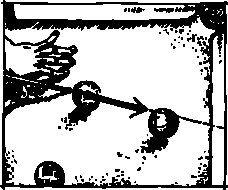
\includegraphics[width=0.6\textwidth]{figures/fig-03-11.pdf}
\caption{Oblique collision between bodies of equal mass.}
\label{fig-3.11}
\end{figure}
Let us consider another example of a collision between
bodies in accordance with the law of elastic collisions,
namely an oblique collision between bodies of equal mass
(\figr{fig-3.11}). The second body was stationary prior to
the collision, so the laws of conservation of momentum
and energy have the form:
\begin{equation*}%
m \mathbf{v_{1}} = m\mathbf{u_{1}}+ m\mathbf{u_{1}}
\end{equation*}
Cancelling the mass, we obtain:
\begin{align*}%
\mathbf{v_{1}} &= \mathbf{u_{1}}+ \mathbf{u_{2}}\\
v_{1}^{2} &= u_{1}^{2} + u_{2}^{2}
\end{align*}

Vector $\mathbf{v_{1}}$ is the vector sum of $\mathbf{u_{1}}$ and $\mathbf{u_{2}}$, but this means
that the lengths of the velocity vectors form a triangle.

What kind of triangle is this? Recall the Pythagorean
theorem. Our second equation is an expression of it.
This means that the velocity triangle must be a right
triangle with hypotenuse $\mathbf{v_{1}}$ and legs $\mathbf{u_{1}}$ and $\mathbf{u_{2}}$. Hence, $\mathbf{u_{1}}$ and $\mathbf{u_{2}}$ form right angles with each other. This interesting result shows that in any oblique elastic collision, bodies of equal mass fly apart at right angles.
